% Created by tikzDevice version 0.12.3 on 2020-01-31 10:06:49
% !TEX encoding = UTF-8 Unicode
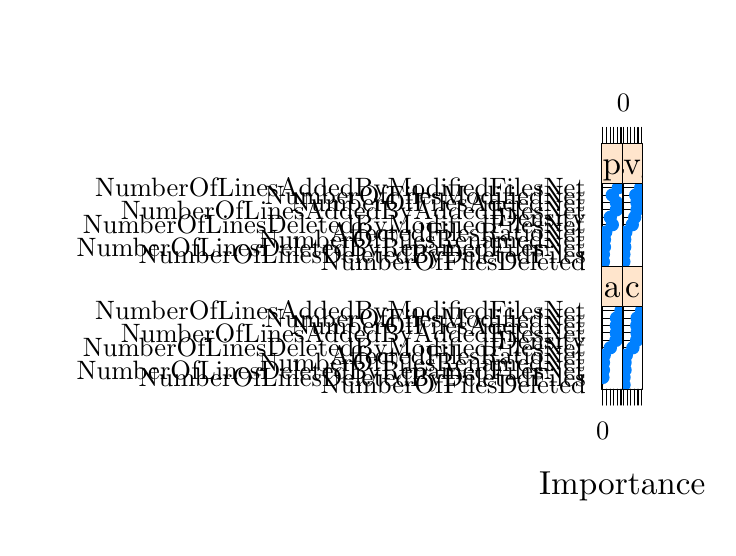
\begin{tikzpicture}[x=1pt,y=1pt]
\definecolor{fillColor}{RGB}{255,255,255}
\path[use as bounding box,fill=fillColor,fill opacity=0.00] (0,0) rectangle (245.72,180.67);
\begin{scope}
\path[clip] (  0.00,  0.00) rectangle (245.72,180.67);

\path[] (  0.00,  0.00) rectangle (245.72,180.68);
\definecolor{drawColor}{RGB}{0,0,0}

\node[text=drawColor,anchor=base,inner sep=0pt, outer sep=0pt, scale=  1.20] at (214.84, 12.05) {Importance};
\end{scope}
\begin{scope}
\path[clip] (  0.00,  0.00) rectangle (245.72,180.67);
\definecolor{drawColor}{RGB}{0,0,0}

\node[text=drawColor,anchor=base east,inner sep=0pt, outer sep=0pt, scale=  0.96] at (201.69, 48.32) {NumberOfFilesDeleted};

\node[text=drawColor,anchor=base east,inner sep=0pt, outer sep=0pt, scale=  0.96] at (201.69, 51.00) {NumberOfLinesDeletedByDeletedFiles};

\node[text=drawColor,anchor=base east,inner sep=0pt, outer sep=0pt, scale=  0.96] at (201.69, 53.67) {NumberOfLinesDeletedByRenamedFilesNet};

\node[text=drawColor,anchor=base east,inner sep=0pt, outer sep=0pt, scale=  0.96] at (201.69, 56.35) {NumberOfFilesRenamedNet};

\node[text=drawColor,anchor=base east,inner sep=0pt, outer sep=0pt, scale=  0.96] at (201.69, 59.03) {AffectedFilesRatioNet};

\node[text=drawColor,anchor=base east,inner sep=0pt, outer sep=0pt, scale=  0.96] at (201.69, 61.71) {NumberOfLinesDeletedByModifiedFilesNet};

\node[text=drawColor,anchor=base east,inner sep=0pt, outer sep=0pt, scale=  0.96] at (201.69, 64.39) {Density};

\node[text=drawColor,anchor=base east,inner sep=0pt, outer sep=0pt, scale=  0.96] at (201.69, 67.07) {NumberOfLinesAddedByAddedFilesNet};

\node[text=drawColor,anchor=base east,inner sep=0pt, outer sep=0pt, scale=  0.96] at (201.69, 69.75) {NumberOfFilesAddedNet};

\node[text=drawColor,anchor=base east,inner sep=0pt, outer sep=0pt, scale=  0.96] at (201.69, 72.42) {NumberOfFilesModifiedNet};

\node[text=drawColor,anchor=base east,inner sep=0pt, outer sep=0pt, scale=  0.96] at (201.69, 75.10) {NumberOfLinesAddedByModifiedFilesNet};
\end{scope}
\begin{scope}
\path[clip] (  0.00,  0.00) rectangle (245.72,180.67);
\definecolor{drawColor}{RGB}{0,0,0}

\path[draw=drawColor,line width= 0.4pt,line join=round,line cap=round] (207.84, 50.02) -- (207.84, 44.32);

\path[draw=drawColor,line width= 0.4pt,line join=round,line cap=round] (209.15, 50.02) -- (209.15, 44.32);

\path[draw=drawColor,line width= 0.4pt,line join=round,line cap=round] (210.46, 50.02) -- (210.46, 44.32);

\path[draw=drawColor,line width= 0.4pt,line join=round,line cap=round] (211.76, 50.02) -- (211.76, 44.32);

\path[draw=drawColor,line width= 0.4pt,line join=round,line cap=round] (213.07, 50.02) -- (213.07, 44.32);

\path[draw=drawColor,line width= 0.4pt,line join=round,line cap=round] (214.38, 50.02) -- (214.38, 44.32);

\node[text=drawColor,anchor=base,inner sep=0pt, outer sep=0pt, scale=  0.96] at (207.84, 32.02) {0};
\end{scope}
\begin{scope}
\path[clip] (207.38, 50.02) rectangle (214.84, 80.02);
\definecolor{drawColor}{RGB}{0,0,0}

\path[draw=drawColor,line width= 0.4pt,line join=round,line cap=round] (207.84, 50.02) -- (207.84, 80.02);

\path[draw=drawColor,line width= 0.4pt,line join=round,line cap=round] (214.38, 78.41) -- (207.84, 78.41);

\path[draw=drawColor,line width= 0.4pt,line join=round,line cap=round] (212.78, 75.73) -- (207.84, 75.73);

\path[draw=drawColor,line width= 0.4pt,line join=round,line cap=round] (212.73, 73.05) -- (207.84, 73.05);

\path[draw=drawColor,line width= 0.4pt,line join=round,line cap=round] (212.73, 70.37) -- (207.84, 70.37);

\path[draw=drawColor,line width= 0.4pt,line join=round,line cap=round] (212.58, 67.69) -- (207.84, 67.69);

\path[draw=drawColor,line width= 0.4pt,line join=round,line cap=round] (210.55, 65.02) -- (207.84, 65.02);

\path[draw=drawColor,line width= 0.4pt,line join=round,line cap=round] (208.34, 62.34) -- (207.84, 62.34);

\path[draw=drawColor,line width= 0.4pt,line join=round,line cap=round] (208.05, 59.66) -- (207.84, 59.66);

\path[draw=drawColor,line width= 0.4pt,line join=round,line cap=round] (208.04, 56.98) -- (207.84, 56.98);

\path[draw=drawColor,line width= 0.4pt,line join=round,line cap=round] (207.84, 54.30) -- (207.84, 54.30);

\path[draw=drawColor,line width= 0.4pt,line join=round,line cap=round] (207.84, 51.62) -- (207.84, 51.62);
\definecolor{fillColor}{RGB}{0,128,255}

\path[fill=fillColor] (214.38, 78.41) circle (  2.41);

\path[fill=fillColor] (212.78, 75.73) circle (  2.41);

\path[fill=fillColor] (212.73, 73.05) circle (  2.41);

\path[fill=fillColor] (212.73, 70.37) circle (  2.41);

\path[fill=fillColor] (212.58, 67.69) circle (  2.41);

\path[fill=fillColor] (210.55, 65.02) circle (  2.41);

\path[fill=fillColor] (208.34, 62.34) circle (  2.41);

\path[fill=fillColor] (208.05, 59.66) circle (  2.41);

\path[fill=fillColor] (208.04, 56.98) circle (  2.41);

\path[fill=fillColor] (207.84, 54.30) circle (  2.41);
\end{scope}
\begin{scope}
\path[clip] (  0.00,  0.00) rectangle (245.72,180.67);
\definecolor{drawColor}{RGB}{0,0,0}

\path[draw=drawColor,line width= 0.4pt,line join=round,line cap=round] (207.38, 50.02) rectangle (214.84, 80.02);
\end{scope}
\begin{scope}
\path[clip] (207.38, 80.02) rectangle (214.84, 94.47);
\definecolor{drawColor}{RGB}{255,229,204}
\definecolor{fillColor}{RGB}{255,229,204}

\path[draw=drawColor,line width= 0.4pt,line join=round,line cap=round,fill=fillColor] (207.38, 80.02) rectangle (214.84, 94.47);
\definecolor{drawColor}{RGB}{0,0,0}

\node[text=drawColor,anchor=base west,inner sep=0pt, outer sep=0pt, scale=  1.20] at (208.11, 83.11) {a};
\end{scope}
\begin{scope}
\path[clip] (  0.00,  0.00) rectangle (245.72,180.67);
\definecolor{drawColor}{RGB}{0,0,0}

\path[draw=drawColor,line width= 0.4pt,line join=round,line cap=round] (207.38, 80.02) rectangle (214.84, 94.47);
\end{scope}
\begin{scope}
\path[clip] (  0.00,  0.00) rectangle (245.72,180.67);
\definecolor{drawColor}{RGB}{0,0,0}

\path[draw=drawColor,line width= 0.4pt,line join=round,line cap=round] (215.29, 50.02) -- (215.29, 44.32);

\path[draw=drawColor,line width= 0.4pt,line join=round,line cap=round] (216.60, 50.02) -- (216.60, 44.32);

\path[draw=drawColor,line width= 0.4pt,line join=round,line cap=round] (217.91, 50.02) -- (217.91, 44.32);

\path[draw=drawColor,line width= 0.4pt,line join=round,line cap=round] (219.22, 50.02) -- (219.22, 44.32);

\path[draw=drawColor,line width= 0.4pt,line join=round,line cap=round] (220.53, 50.02) -- (220.53, 44.32);

\path[draw=drawColor,line width= 0.4pt,line join=round,line cap=round] (221.83, 50.02) -- (221.83, 44.32);
\end{scope}
\begin{scope}
\path[clip] (214.84, 50.02) rectangle (222.29, 80.02);
\definecolor{drawColor}{RGB}{0,0,0}

\path[draw=drawColor,line width= 0.4pt,line join=round,line cap=round] (215.29, 50.02) -- (215.29, 80.02);

\path[draw=drawColor,line width= 0.4pt,line join=round,line cap=round] (221.83, 78.41) -- (215.29, 78.41);

\path[draw=drawColor,line width= 0.4pt,line join=round,line cap=round] (220.23, 75.73) -- (215.29, 75.73);

\path[draw=drawColor,line width= 0.4pt,line join=round,line cap=round] (220.09, 73.05) -- (215.29, 73.05);

\path[draw=drawColor,line width= 0.4pt,line join=round,line cap=round] (220.18, 70.37) -- (215.29, 70.37);

\path[draw=drawColor,line width= 0.4pt,line join=round,line cap=round] (220.04, 67.69) -- (215.29, 67.69);

\path[draw=drawColor,line width= 0.4pt,line join=round,line cap=round] (218.70, 65.02) -- (215.29, 65.02);

\path[draw=drawColor,line width= 0.4pt,line join=round,line cap=round] (216.32, 62.34) -- (215.29, 62.34);

\path[draw=drawColor,line width= 0.4pt,line join=round,line cap=round] (215.86, 59.66) -- (215.29, 59.66);

\path[draw=drawColor,line width= 0.4pt,line join=round,line cap=round] (215.86, 56.98) -- (215.29, 56.98);

\path[draw=drawColor,line width= 0.4pt,line join=round,line cap=round] (215.49, 54.30) -- (215.29, 54.30);

\path[draw=drawColor,line width= 0.4pt,line join=round,line cap=round] (215.49, 51.62) -- (215.29, 51.62);
\definecolor{fillColor}{RGB}{0,128,255}

\path[fill=fillColor] (221.83, 78.41) circle (  2.41);

\path[fill=fillColor] (220.23, 75.73) circle (  2.41);

\path[fill=fillColor] (220.09, 73.05) circle (  2.41);

\path[fill=fillColor] (220.18, 70.37) circle (  2.41);

\path[fill=fillColor] (220.04, 67.69) circle (  2.41);

\path[fill=fillColor] (218.70, 65.02) circle (  2.41);

\path[fill=fillColor] (216.32, 62.34) circle (  2.41);

\path[fill=fillColor] (215.86, 59.66) circle (  2.41);

\path[fill=fillColor] (215.86, 56.98) circle (  2.41);

\path[fill=fillColor] (215.49, 54.30) circle (  2.41);

\path[fill=fillColor] (215.49, 51.62) circle (  2.41);
\end{scope}
\begin{scope}
\path[clip] (  0.00,  0.00) rectangle (245.72,180.67);
\definecolor{drawColor}{RGB}{0,0,0}

\path[draw=drawColor,line width= 0.4pt,line join=round,line cap=round] (214.84, 50.02) rectangle (222.29, 80.02);
\end{scope}
\begin{scope}
\path[clip] (214.84, 80.02) rectangle (222.29, 94.47);
\definecolor{drawColor}{RGB}{255,229,204}
\definecolor{fillColor}{RGB}{255,229,204}

\path[draw=drawColor,line width= 0.4pt,line join=round,line cap=round,fill=fillColor] (214.84, 80.02) rectangle (222.29, 94.47);
\definecolor{drawColor}{RGB}{0,0,0}

\node[text=drawColor,anchor=base west,inner sep=0pt, outer sep=0pt, scale=  1.20] at (215.90, 83.11) {c};
\end{scope}
\begin{scope}
\path[clip] (  0.00,  0.00) rectangle (245.72,180.67);
\definecolor{drawColor}{RGB}{0,0,0}

\path[draw=drawColor,line width= 0.4pt,line join=round,line cap=round] (214.84, 80.02) rectangle (222.29, 94.47);
\end{scope}
\begin{scope}
\path[clip] (  0.00,  0.00) rectangle (245.72,180.67);
\definecolor{drawColor}{RGB}{0,0,0}

\path[draw=drawColor,line width= 0.4pt,line join=round,line cap=round] (207.84,138.92) -- (207.84,144.61);

\path[draw=drawColor,line width= 0.4pt,line join=round,line cap=round] (209.15,138.92) -- (209.15,144.61);

\path[draw=drawColor,line width= 0.4pt,line join=round,line cap=round] (210.46,138.92) -- (210.46,144.61);

\path[draw=drawColor,line width= 0.4pt,line join=round,line cap=round] (211.76,138.92) -- (211.76,144.61);

\path[draw=drawColor,line width= 0.4pt,line join=round,line cap=round] (213.07,138.92) -- (213.07,144.61);

\path[draw=drawColor,line width= 0.4pt,line join=round,line cap=round] (214.38,138.92) -- (214.38,144.61);
\end{scope}
\begin{scope}
\path[clip] (  0.00,  0.00) rectangle (245.72,180.67);
\definecolor{drawColor}{RGB}{0,0,0}

\node[text=drawColor,anchor=base east,inner sep=0pt, outer sep=0pt, scale=  0.96] at (201.69, 92.77) {NumberOfFilesDeleted};

\node[text=drawColor,anchor=base east,inner sep=0pt, outer sep=0pt, scale=  0.96] at (201.69, 95.45) {NumberOfLinesDeletedByDeletedFiles};

\node[text=drawColor,anchor=base east,inner sep=0pt, outer sep=0pt, scale=  0.96] at (201.69, 98.13) {NumberOfLinesDeletedByRenamedFilesNet};

\node[text=drawColor,anchor=base east,inner sep=0pt, outer sep=0pt, scale=  0.96] at (201.69,100.81) {NumberOfFilesRenamedNet};

\node[text=drawColor,anchor=base east,inner sep=0pt, outer sep=0pt, scale=  0.96] at (201.69,103.49) {AffectedFilesRatioNet};

\node[text=drawColor,anchor=base east,inner sep=0pt, outer sep=0pt, scale=  0.96] at (201.69,106.16) {NumberOfLinesDeletedByModifiedFilesNet};

\node[text=drawColor,anchor=base east,inner sep=0pt, outer sep=0pt, scale=  0.96] at (201.69,108.84) {Density};

\node[text=drawColor,anchor=base east,inner sep=0pt, outer sep=0pt, scale=  0.96] at (201.69,111.52) {NumberOfLinesAddedByAddedFilesNet};

\node[text=drawColor,anchor=base east,inner sep=0pt, outer sep=0pt, scale=  0.96] at (201.69,114.20) {NumberOfFilesAddedNet};

\node[text=drawColor,anchor=base east,inner sep=0pt, outer sep=0pt, scale=  0.96] at (201.69,116.88) {NumberOfFilesModifiedNet};

\node[text=drawColor,anchor=base east,inner sep=0pt, outer sep=0pt, scale=  0.96] at (201.69,119.56) {NumberOfLinesAddedByModifiedFilesNet};
\end{scope}
\begin{scope}
\path[clip] (207.38, 94.47) rectangle (214.84,124.47);
\definecolor{drawColor}{RGB}{0,0,0}

\path[draw=drawColor,line width= 0.4pt,line join=round,line cap=round] (207.84, 94.47) -- (207.84,124.47);

\path[draw=drawColor,line width= 0.4pt,line join=round,line cap=round] (213.45,122.86) -- (207.84,122.86);

\path[draw=drawColor,line width= 0.4pt,line join=round,line cap=round] (211.25,120.18) -- (207.84,120.18);

\path[draw=drawColor,line width= 0.4pt,line join=round,line cap=round] (212.73,117.51) -- (207.84,117.51);

\path[draw=drawColor,line width= 0.4pt,line join=round,line cap=round] (212.72,114.83) -- (207.84,114.83);

\path[draw=drawColor,line width= 0.4pt,line join=round,line cap=round] (210.53,112.15) -- (207.84,112.15);

\path[draw=drawColor,line width= 0.4pt,line join=round,line cap=round] (211.25,109.47) -- (207.84,109.47);

\path[draw=drawColor,line width= 0.4pt,line join=round,line cap=round] (208.86,106.79) -- (207.84,106.79);

\path[draw=drawColor,line width= 0.4pt,line join=round,line cap=round] (208.41,104.11) -- (207.84,104.11);

\path[draw=drawColor,line width= 0.4pt,line join=round,line cap=round] (208.40,101.43) -- (207.84,101.43);

\path[draw=drawColor,line width= 0.4pt,line join=round,line cap=round] (208.03, 98.76) -- (207.84, 98.76);

\path[draw=drawColor,line width= 0.4pt,line join=round,line cap=round] (208.03, 96.08) -- (207.84, 96.08);
\definecolor{fillColor}{RGB}{0,128,255}

\path[fill=fillColor] (213.45,122.86) circle (  2.41);

\path[fill=fillColor] (211.25,120.18) circle (  2.41);

\path[fill=fillColor] (212.73,117.51) circle (  2.41);

\path[fill=fillColor] (212.72,114.83) circle (  2.41);

\path[fill=fillColor] (210.53,112.15) circle (  2.41);

\path[fill=fillColor] (211.25,109.47) circle (  2.41);

\path[fill=fillColor] (208.86,106.79) circle (  2.41);

\path[fill=fillColor] (208.41,104.11) circle (  2.41);

\path[fill=fillColor] (208.40,101.43) circle (  2.41);

\path[fill=fillColor] (208.03, 98.76) circle (  2.41);

\path[fill=fillColor] (208.03, 96.08) circle (  2.41);
\end{scope}
\begin{scope}
\path[clip] (  0.00,  0.00) rectangle (245.72,180.67);
\definecolor{drawColor}{RGB}{0,0,0}

\path[draw=drawColor,line width= 0.4pt,line join=round,line cap=round] (207.38, 94.47) rectangle (214.84,124.47);
\end{scope}
\begin{scope}
\path[clip] (207.38,124.47) rectangle (214.84,138.92);
\definecolor{drawColor}{RGB}{255,229,204}
\definecolor{fillColor}{RGB}{255,229,204}

\path[draw=drawColor,line width= 0.4pt,line join=round,line cap=round,fill=fillColor] (207.38,124.47) rectangle (214.84,138.92);
\definecolor{drawColor}{RGB}{0,0,0}

\node[text=drawColor,anchor=base west,inner sep=0pt, outer sep=0pt, scale=  1.20] at (207.78,127.56) {p};
\end{scope}
\begin{scope}
\path[clip] (  0.00,  0.00) rectangle (245.72,180.67);
\definecolor{drawColor}{RGB}{0,0,0}

\path[draw=drawColor,line width= 0.4pt,line join=round,line cap=round] (207.38,124.47) rectangle (214.84,138.92);
\end{scope}
\begin{scope}
\path[clip] (  0.00,  0.00) rectangle (245.72,180.67);
\definecolor{drawColor}{RGB}{0,0,0}

\path[draw=drawColor,line width= 0.4pt,line join=round,line cap=round] (215.29,138.92) -- (215.29,144.61);

\path[draw=drawColor,line width= 0.4pt,line join=round,line cap=round] (216.60,138.92) -- (216.60,144.61);

\path[draw=drawColor,line width= 0.4pt,line join=round,line cap=round] (217.91,138.92) -- (217.91,144.61);

\path[draw=drawColor,line width= 0.4pt,line join=round,line cap=round] (219.22,138.92) -- (219.22,144.61);

\path[draw=drawColor,line width= 0.4pt,line join=round,line cap=round] (220.53,138.92) -- (220.53,144.61);

\path[draw=drawColor,line width= 0.4pt,line join=round,line cap=round] (221.83,138.92) -- (221.83,144.61);

\node[text=drawColor,anchor=base,inner sep=0pt, outer sep=0pt, scale=  0.96] at (215.29,150.31) {0};
\end{scope}
\begin{scope}
\path[clip] (214.84, 94.47) rectangle (222.29,124.47);
\definecolor{drawColor}{RGB}{0,0,0}

\path[draw=drawColor,line width= 0.4pt,line join=round,line cap=round] (215.29, 94.47) -- (215.29,124.47);

\path[draw=drawColor,line width= 0.4pt,line join=round,line cap=round] (221.52,122.86) -- (215.29,122.86);

\path[draw=drawColor,line width= 0.4pt,line join=round,line cap=round] (219.72,120.18) -- (215.29,120.18);

\path[draw=drawColor,line width= 0.4pt,line join=round,line cap=round] (220.15,117.51) -- (215.29,117.51);

\path[draw=drawColor,line width= 0.4pt,line join=round,line cap=round] (220.18,114.83) -- (215.29,114.83);

\path[draw=drawColor,line width= 0.4pt,line join=round,line cap=round] (219.35,112.15) -- (215.29,112.15);

\path[draw=drawColor,line width= 0.4pt,line join=round,line cap=round] (218.47,109.47) -- (215.29,109.47);

\path[draw=drawColor,line width= 0.4pt,line join=round,line cap=round] (216.14,106.79) -- (215.29,106.79);

\path[draw=drawColor,line width= 0.4pt,line join=round,line cap=round] (215.74,104.11) -- (215.29,104.11);

\path[draw=drawColor,line width= 0.4pt,line join=round,line cap=round] (215.74,101.43) -- (215.29,101.43);

\path[draw=drawColor,line width= 0.4pt,line join=round,line cap=round] (215.43, 98.76) -- (215.29, 98.76);

\path[draw=drawColor,line width= 0.4pt,line join=round,line cap=round] (215.42, 96.08) -- (215.29, 96.08);
\definecolor{fillColor}{RGB}{0,128,255}

\path[fill=fillColor] (221.52,122.86) circle (  2.41);

\path[fill=fillColor] (219.72,120.18) circle (  2.41);

\path[fill=fillColor] (220.15,117.51) circle (  2.41);

\path[fill=fillColor] (220.18,114.83) circle (  2.41);

\path[fill=fillColor] (219.35,112.15) circle (  2.41);

\path[fill=fillColor] (218.47,109.47) circle (  2.41);

\path[fill=fillColor] (216.14,106.79) circle (  2.41);

\path[fill=fillColor] (215.74,104.11) circle (  2.41);

\path[fill=fillColor] (215.74,101.43) circle (  2.41);

\path[fill=fillColor] (215.43, 98.76) circle (  2.41);

\path[fill=fillColor] (215.42, 96.08) circle (  2.41);
\end{scope}
\begin{scope}
\path[clip] (  0.00,  0.00) rectangle (245.72,180.67);
\definecolor{drawColor}{RGB}{0,0,0}

\path[draw=drawColor,line width= 0.4pt,line join=round,line cap=round] (214.84, 94.47) rectangle (222.29,124.47);
\end{scope}
\begin{scope}
\path[clip] (214.84,124.47) rectangle (222.29,138.92);
\definecolor{drawColor}{RGB}{255,229,204}
\definecolor{fillColor}{RGB}{255,229,204}

\path[draw=drawColor,line width= 0.4pt,line join=round,line cap=round,fill=fillColor] (214.84,124.47) rectangle (222.29,138.92);
\definecolor{drawColor}{RGB}{0,0,0}

\node[text=drawColor,anchor=base west,inner sep=0pt, outer sep=0pt, scale=  1.20] at (209.57,127.56) {avg};
\end{scope}
\begin{scope}
\path[clip] (  0.00,  0.00) rectangle (245.72,180.67);
\definecolor{drawColor}{RGB}{0,0,0}

\path[draw=drawColor,line width= 0.4pt,line join=round,line cap=round] (214.84,124.47) rectangle (222.29,138.92);
\end{scope}
\end{tikzpicture}
